\documentclass[11pt, a4paper]{article}
\usepackage[utf8]{inputenc}
\usepackage{minted}
\usepackage{graphicx}
\usepackage{hyperref}
\usepackage{subcaption}
\graphicspath{{./images/}}


\begin{document}
\title{Behavioral Cloning Project}
\author{Samuel Navarro}
\date{\today}
\maketitle
	
\tableofcontents{}


\section{Model Architecture and Training Strategy}%
\label{sec:model_architecture_and_training_strategy}

\subsection{An appropriate model architecture has been employed}%
\label{sub:an_appropriate_model_architecture_has_been_employed}


My model is similar to the one used in \href{http://images.nvidia.com/content/tegra/automotive/images/2016/solutions/pdf/end-to-end-dl-using-px.pdf}{NVIDIA}. It consists of a convolutional neural network with 5x5 kernel size for the 3 first layers. Here I used a depth between 24 and 48. After that, I used two more convolutional layers with 3x3 of kernel size and 64 number of filters (depth). Then I used 5 more fully connected layers. With Dropout of 0.5 after the second fully connected layer and 0.25 after the fourth fully connected layer. This is in \texttt{model.py} in lines 70-84.  

The model include RELU activations to introduce nonlinearity and the data is normalized in the model using a Keras lambda layer. The data is also Cropped to reduce noise. I cropped 60 pixels from above the image and 25 from below. I didn't cropped pixels from the sides. 

The reason why I used those values was to simply cut off the sky in the image.

\subsection{Attempts to reduce overfitting the model}%
\label{sub:attempts_to_reduce_overfitting_th_emodel}

The model contains dropout layers with \texttt{p=0.5}  after the second fully connected layer and \texttt{p=0.25} after the fourth fully connected layer. ( lines 80 and 83 in \texttt{model.py})  


\subsection{Model parameter tuning}%
\label{sub:model_parameter_tuning}

The model used an Adam optimizer so the learning rate was not tuned manually. (line 87 in \texttt{model.py})




\subsection{Appropriate Training Data}%
\label{sub:appropiate_training_data}

Training data was chosen from the simulator. I repeatedly play the simulator in order to obtain data with good quality and from different angles. I play the simulator several times in order to be confortable with it so I can obtain data with the car in the center of the road as long as possible.


The data was collected in 3 ways:
\begin{enumerate}
	\item Driving Clockwise on both tracks.
	\item Driving Counter-Clockwise on both tracks.
	\item Again in segments when the model find difficult to keep on the middle of the road.
\end{enumerate}

To perform the third point, I played the simulator in Autonomous mode and when I found that the model was having trouble to stay on track, I played the simulator in Training Mode just in that particular segment.


Here's an example image of center lane driving:


\begin{figure}[htpb!]
	\centering
	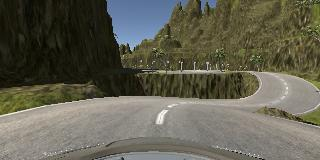
\includegraphics[width=0.8\linewidth]{center_example}
	\caption{Center Example}
	\label{fig:center_example}
\end{figure}



Another thing I used to get more data was to flip the images. 

The Figure~\ref{fig:data_augmentation} shows the original and the flipped image.



\begin{figure}[htpb!]
 
\begin{subfigure}{0.5\textwidth}
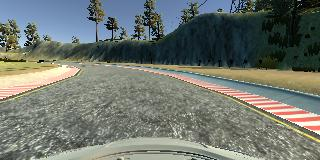
\includegraphics[width=0.9\linewidth, height=5cm]{original} 
\caption{Original}
\label{fig:original}
\end{subfigure}
\begin{subfigure}{0.5\textwidth}
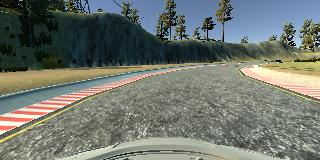
\includegraphics[width=0.9\linewidth, height=5cm]{flipped}
\caption{Flipped}
\label{fig:subim2}
\end{subfigure}
 
\caption{Data Augmentation}
\label{fig:data_augmentation}
\end{figure}



\subsection{Final Model Architecture}%
\label{sub:final_model_architecture}



I decided to start with the model used in NVIDIA, simply because that had been tested in the past. At the beginning, my model doing good in the training set but it had a poor performance with the validations samples so I added the two dropout layers. After that the model started to perform almost the same in the two samples. 

The data was splited in three sets:
\begin{itemize}
	\item Training set: 80 \% of the data 
	\item Validation set: 18 \% of the data
	\item Test set: 2 \% of the data
\end{itemize}




The number of epochs was 8. This seemed obvious after we take a look at the validation and training loss plots in the Figure~\ref{fig:loss}

\begin{figure}[htpb!]
	\centering
	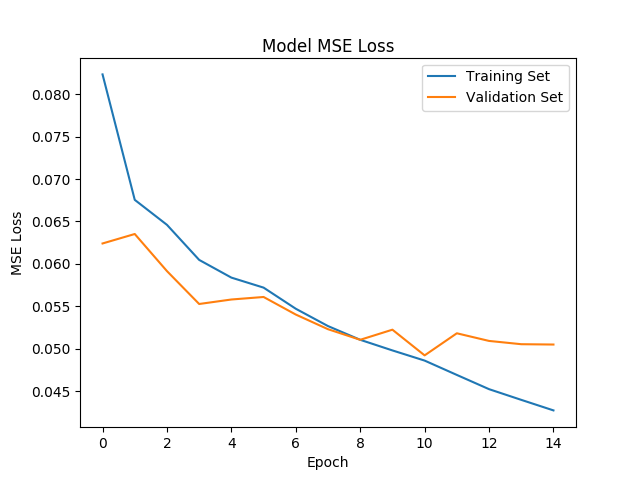
\includegraphics[width=0.8\linewidth]{loss}
	\caption{Loss}
	\label{fig:loss}
\end{figure}

With this plot we can see that is likely to overfitt the training data if we continue to train.




The final model architecture (lines 71-85 of \texttt{model.py}) was mentioned in the Section \ref{sub:an_appropriate_model_architecture_has_been_employed}

The visualization of the architecture is in Figure~\ref{fig:model_plot}

\begin{figure}[htpb!]
	\centering
	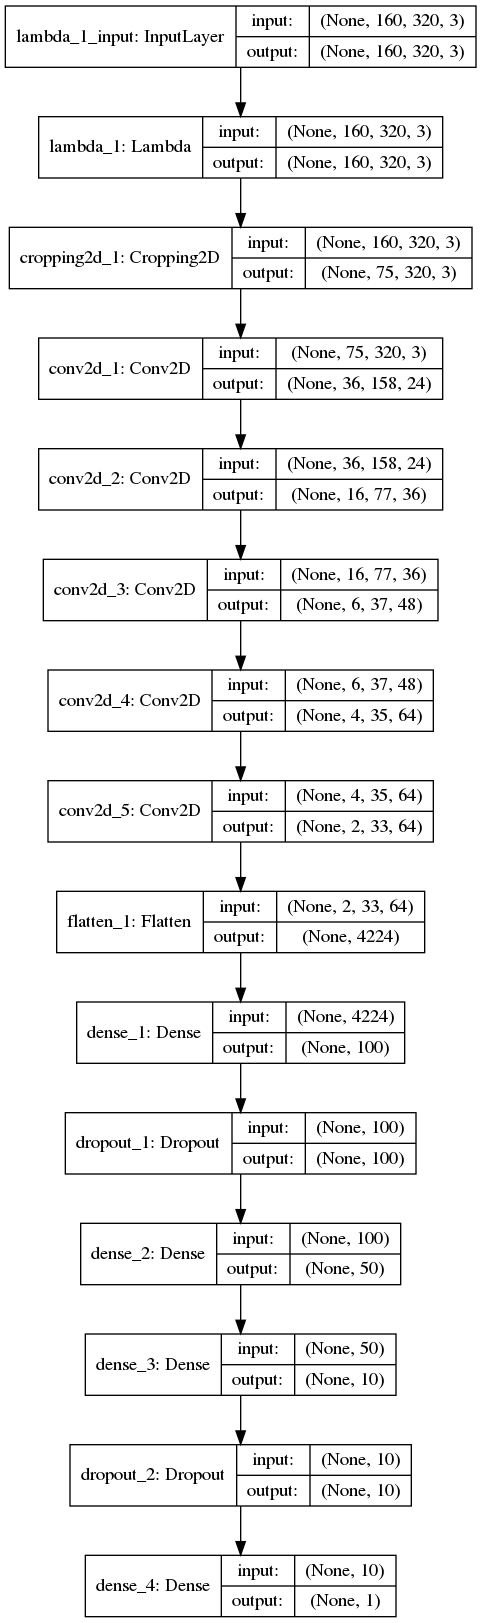
\includegraphics[height=0.8\linewidth]{model_plot}
	\caption{Model Plot}
	\label{fig:model_plot}
\end{figure}



\subsection{Test set}%
\label{sub:test_set}


The best model was taken from the checkpoint (line 90 \texttt{model.py}) and we picked the model with the lowest \textbf{val\_loss}. \\

The result of this model was \textbf{val\_loss: 0.0492}. The loss in the \textbf{test set was 0.0489.}


But, I believed that driving the car in \textbf{autonomous} mode was kind of cheating because the model had already seen the images. Because of that, I tried to drive the car in another Roadway apart from the jungle and the lake tracks that you guys provide us.

I took \href{https://assetstore.unity.com/?category=3d%2Fenvironments%2Froadways&orderBy=1}{This one} from the unity asset store.


When I tested the model in this new environment I was impressed for how good the model was performing.


In the Figure~\ref{fig:newtrack} is the output of the model in a new track.

\begin{figure}[htpb!]
	\centering
	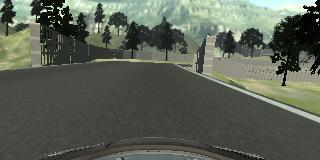
\includegraphics[width=0.8\linewidth]{newtrack}
	\caption{New track}
	\label{fig:newtrack}
\end{figure}




\end{document}
